% =========================================================================
%  P4 -- Adaptive security for federated agentic MEC
%  IEEEtran journal manuscript.  Result tables are \input, never retyped.
% =========================================================================
\documentclass[journal,10pt]{IEEEtran}

\usepackage[utf8]{inputenc}
\usepackage[T1]{fontenc}
\usepackage{amsmath,amssymb,amsthm}
\usepackage{graphicx}
\usepackage{booktabs}
\usepackage{multirow}
\usepackage{array}
\usepackage{subcaption}
\usepackage{algorithm}
\usepackage{algpseudocode}
\usepackage{url}
\usepackage{cite}
\usepackage{xcolor}
\usepackage{tikz}
\usepackage{balance}
\usetikzlibrary{positioning,arrows.meta,fit,calc,shapes.geometric}

\graphicspath{{../results/figures/}{diagrams/}}

\newtheorem{proposition}{Proposition}
\newcommand{\bigO}{\ensuremath{\mathcal{O}}}

\hyphenation{post-quan-tum cryp-to-graph-ic ag-gre-ga-tion Pure-Edge-Sim }

\begin{document}

\title{Cost-Aware Adaptive Security for Federated Agentic Edge Computing:
Trading Cryptographic Level against Deadline}

\author{Anonymous Authors%
\thanks{Manuscript prepared for review. Security parameters are
literature-calibrated and every result table is generated from the released
artifact.}}

\markboth{IEEE Transactions on Mobile Computing (submitted)}%
{Cost-Aware Adaptive Security for Federated Agentic Edge Computing}

\maketitle

\begin{abstract}
Edge deployments that run federated learning for agentic services must choose a
cryptographic profile per exchange: no protection, a post-quantum signature, a
post-quantum channel, homomorphic encryption, or secure aggregation. The
literature usually evaluates one profile at a time, which hides the fact that
the profiles differ by more than an order of magnitude in delay. We formalise
five profiles from NIST FIPS 203/204, CKKS and secure aggregation, attach
literature-calibrated compute and payload multipliers to each, and add an
adversarial model with poisoning, eavesdropping and membership-inference
components. We then evaluate an orchestrator that selects the profile and the
host jointly, subject to a deadline and a per-tier risk target. Across $680$
seeded runs, unconditional maximum security costs $+107.9\%$ delay and
$2.06\times$ byte amplification, while the unprotected baseline suffers a
$0.415$ composite attack rate. The adaptive policy reaches a $0.126$ attack
rate at $+3.7\%$ delay: $69.6\%$ of the attack reduction of maximum security for
$3.4\%$ of its delay cost. It is Pareto-optimal rather than dominant---static
maximum security achieves higher protected utility ($0.970$ versus $0.874$) and
we say so---and it strictly dominates the two middle static profiles on both
delay and utility. A threat sweep from $\tau=0$ to $0.4$, load and model-size
sweeps, and an overhead decomposition bound where the policy remains usable.
\end{abstract}

\begin{IEEEkeywords}
Edge computing, federated learning, post-quantum cryptography, homomorphic
encryption, secure aggregation, adaptive security, membership inference.
\end{IEEEkeywords}

% =========================================================================
\section{Introduction}
\label{sec:intro}

A federated learning round at the edge carries model updates, not user data,
and that is often presented as the privacy solution. It is not. Updates leak
training data to membership-inference attacks~\cite{shokri2017membership}, can
be poisoned by a malicious participant~\cite{biggio2012poisoning}, and travel
over links that an eavesdropper can observe. The defences are known: digital
signatures for integrity, key encapsulation for confidentiality,
homomorphic encryption for computation on ciphertext, and secure aggregation
for masked summation~\cite{bonawitz2017secagg,cheon2017ckks}. What is not known
is \emph{which} of them to apply to a given exchange at a given moment.

Current practice applies one profile uniformly. Either the deployment is
``secure'', in which case every exchange pays for homomorphic encryption and
secure aggregation, or it is a prototype, in which case nothing is protected.
Both choices are indefensible at the edge, where the tightest deadline might be
$20$~ms and the cryptographic overhead of the strongest profile is measured in
hundreds of milliseconds. A uniform profile either violates deadlines or
over-protects exchanges that carry nothing sensitive.

This paper treats the profile as a per-task decision, jointly with the placement
decision. The idea is simple: an exchange between a device and a co-located edge
aggregator is exposed to fewer observers than an exchange that crosses the
shared WAN, so it can be protected less; a federated round that carries a model
update is more sensitive than a telemetry read, so it should be protected more;
and a task with a $20$~ms deadline cannot afford a profile whose handshake alone
is $22$~ms. An orchestrator that knows the threat level, the exposure of the
chosen path, and the task's budget can choose a profile that is adequate rather
than maximal.

\subsection{What the results say, including the inconvenient part}
We implement five profiles and an adaptive policy on the Python port of
PureEdgeSim, with an adversarial model whose parameters come from the
literature rather than from the simulator. The results are best read as a
trade-off frontier.

Maximum security (L4: post-quantum channel, homomorphic encryption, secure
aggregation, and clipping) reduces the composite attack rate to $0.019$ but
costs $+107.9\%$ delay and $2.06\times$ byte amplification relative to no
protection. No protection has a $0.415$ attack rate. The adaptive policy sits
between them: attack rate $0.126$, delay overhead $+3.7\%$, byte amplification
$1.23\times$. In terms of protected utility---success ratio times one minus
attack rate---adaptive reaches $0.874$ against $0.580$ for no protection and
$0.970$ for maximum security.

The honest reading is that \textbf{adaptive does not win uniformly}. On
protected utility, both L3 ($0.931$) and L4 ($0.970$) beat it. What adaptive
does is occupy a point that no static profile occupies: it is faster than every
profile that achieves a comparable attack rate, and it dominates the two middle
profiles (L1, L2) outright---better delay \emph{and} better utility. In the
delay--utility plane it is on the Pareto front; on utility alone it is third.

We state this plainly because the alternative---comparing adaptive only against
the unprotected baseline---would produce a flattering and misleading result. The
contribution is a frontier, not a winner.

\subsection{Contributions}
\begin{enumerate}
\item A literature-calibrated matrix of five security profiles with explicit
  provenance (NIST FIPS 203/204, CKKS, secure aggregation), so that the
  overhead numbers can be checked against their sources rather than taken on
  trust (Section~\ref{sec:model}).
\item An adversarial model with three attack channels and a composite
  probability, together with a protected-utility metric that makes the
  security--performance trade explicit (Section~\ref{sec:model}).
\item An orchestrator that selects the profile and the host jointly under a
  deadline constraint and a per-tier risk target, with a preference for
  edge-local aggregation of federated rounds (Section~\ref{sec:method}).
\item A $680$-run evaluation with threat, load and model-size sweeps, paired
  non-parametric statistics, and a Pareto analysis that states where the
  policy wins and where it loses (Section~\ref{sec:res}).
\item A threats-to-validity analysis that separates modelled overhead from
  formal security guarantees (Section~\ref{sec:threats}).
\end{enumerate}

% =========================================================================
\section{Related Work}
\label{sec:related}

\subsection{Post-quantum and privacy-preserving primitives}
NIST standardised ML-KEM (FIPS 203) and ML-DSA (FIPS 204) in 2024, giving
deployable key encapsulation and signatures whose costs are documented in the
standards~\cite{fips203,fips204}. Homomorphic encryption for approximate
arithmetic~\cite{cheon2017ckks} makes it possible to aggregate encrypted updates
but multiplies ciphertext size. Secure aggregation~\cite{bonawitz2017secagg}
masks individual updates so that only the sum is revealed, at the cost of an
extra round of key agreement. Byzantine-robust aggregation~\cite{blanchard2017byzantine}
and clipping bound the influence of poisoned updates. Each primitive has a
measured cost and a measured guarantee; the question we address is how to
compose them per exchange.

\subsection{Federated learning at the edge}
Federated learning was introduced as communication-efficient distributed
training~\cite{mcmahan2017fl} and has since accumulated a literature on
fairness, robustness and privacy~\cite{kairouz2021fl}. Membership
inference~\cite{shokri2017membership} and poisoning~\cite{biggio2012poisoning}
are the two canonical attacks; our model includes both, plus passive
eavesdropping, because a wireless edge link exposes all three. The 2026 corpus
contributes secure offloading with constrained federated
reinforcement learning~\cite{wang2026craft}, quantum-native far-edge
architectures for industrial digital twins~\cite{sammartino2026qfe}, and
secure agentic AI for 6G~\cite{gaba2026secureagentic}. These works argue that
security must be designed in; we argue that it must also be \emph{dosed}.

\subsection{Adaptive and risk-aware security}
Risk-aware security is established in systems security but rare in edge
orchestration. The dependable-computing taxonomy~\cite{avizienis2004dependable}
distinguishes threats, faults and failures in a way that maps cleanly onto our
three attack channels. Our contribution is to make the level a decision
variable of the placement problem rather than a configuration constant.

\subsection{Positioning}
To our knowledge, no prior edge study reports the full delay--utility frontier
of the five standard profiles on one workload, with the adaptive policy placed
on the same axes. That frontier, rather than the adaptive policy alone, is the
result.

% =========================================================================
\section{Security and Adversary Model}
\label{sec:model}

\subsection{Security profiles}
Table~\ref{tab:p4-crypto} lists the five profiles. Each is described by a
compute multiplier and a fixed cryptographic instruction count, a payload
multiplier and a fixed per-message overhead, a container multiplier, a
handshake latency, and three defence factors: integrity (against poisoning),
confidentiality (against eavesdropping), and privacy (against
membership inference). The multipliers were calibrated from the standards and
from the cited systems papers; the table names the source of each row, which is
the minimum a reader needs in order to disagree with a number.

\begin{table*}[t]
\centering
\footnotesize
\caption{Calibrated post-quantum and privacy-preserving security profiles.
Compute and payload are a multiplier plus a fixed per-message cost; container is
a multiplier on the application image; defence gives the integrity,
confidentiality and privacy factors of Section~\ref{sec:model}. Sources are
given per row.}
\label{tab:p4-crypto}
\setlength{\tabcolsep}{5pt}
\begin{tabular}{@{}l l l l c c l@{}}
\toprule
Level & Compute & Payload & Container & Handshake (s) & Defence (I/C/P) & Source\\
\midrule
L0 & 1.00x + 0 MI & 1.00x + 0.0 kB & 1.00x & 0.000 & 0.00/0.00/0.00 & ---\\
L1 & 1.08x + 450 MI & 1.04x + 5.2 kB & 1.05x & 0.002 & 0.55/0.05/0.10 & \cite{fips204,wang2026craft}\\
L2 & 1.24x + 1150 MI & 1.22x + 12.0 kB & 1.15x & 0.006 & 0.72/0.92/0.45 & \cite{fips203,fips204,sammartino2026qfe}\\
L3 & 1.55x + 2600 MI & 1.65x + 28.0 kB & 1.32x & 0.014 & 0.85/0.97/0.86 & \cite{cheon2017ckks,wang2026craft}\\
L4 & 1.85x + 4200 MI & 2.05x + 45.0 kB & 1.55x & 0.022 & 0.96/0.99/0.95 & \cite{bonawitz2017secagg,sammartino2026qfe}\\
\bottomrule
\end{tabular}
\par\vspace{2pt}{\footnotesize\raggedright
I/C/P = integrity (poisoning), confidentiality (eavesdropping) and privacy
(membership-inference) defence factors. L1 is ML-DSA-65; L2 is ML-KEM-768 with
ML-DSA-65 or CSIDH-512 framing; L3 adds CKKS approximate HE at $N=2^{13}$; L4
adds pairwise-masked secure aggregation with norm and cosine clipping.\par}
\end{table*}


Two properties of the table drive everything that follows. First, the cost is
\emph{not linear} in protection: moving from L0 to L1 costs $8\%$ compute, while
moving from L3 to L4 costs a further $19\%$ plus $1{,}600$~MI and $17$~kB per
message. Second, the defence factors are \emph{not proportional} to the cost:
L4 buys $0.96/0.99/0.95$ against L3's $0.85/0.97/0.86$, an eleven-point gain in
integrity and nine in privacy for roughly a third more delay. The frontier is
therefore concave, which is what makes a per-task choice worthwhile.

\subsection{Threat model}
A threat intensity $\tau\in[0,1]$ parameterises the adversary's capability. For
a task executed at a node with tier exposure $\epsilon\in[0,1]$, profile
$\ell$, and model-update size scale $s$, the three channel probabilities are
\begin{align}
p_{\text{poison}} &= \tau\,(1-I_\ell), \label{eq:poison}\\
p_{\text{eaves}}  &= \tau\,\epsilon\,(1-C_\ell), \label{eq:eaves}\\
p_{\text{leak}}   &= \beta(\tau,s)\,(0.65+0.35\epsilon)\,(1-P_\ell),
\label{eq:leak}
\end{align}
where $I_\ell,C_\ell,P_\ell$ are the integrity, confidentiality and privacy
defence factors of profile $\ell$, and
$\beta(\tau,s)=\min(0.5,(0.18+0.32\tau)(0.85+0.15\min(s,4)))$ is the base
membership-inference leakage. The composite attack probability is
\begin{equation}
p_{\text{attack}}=1-(1-p_{\text{poison}})(1-p_{\text{eaves}})(1-p_{\text{leak}}).
\label{eq:composite}
\end{equation}
The form of \eqref{eq:composite} matters: the channels are treated as
independent opportunities, so the composite is dominated by the largest channel
and cannot be driven to zero by fixing one of them. That is why L1, which
largely fixes integrity, still leaves a $0.315$ composite rate at
$\tau=0.2$.

Edge co-location reduces exposure: an exchange that terminates at an edge
aggregation point is modelled with a lower $\epsilon$ than one that crosses the
shared WAN, and the aggregation point also earns a small bonus to all three
defence factors because the aggregator applies platform-level hardening. This
is the mechanism behind the orchestrator's preference for edge-local
aggregation.

\subsection{Utility}
We report \emph{protected utility}
\begin{equation}
U=\text{success ratio}\times(1-\overline{p_{\text{attack}}}),
\label{eq:utility}
\end{equation}
where the bar is the mean over tasks. The product is deliberately harsh: a
policy that serves everything insecurely and a policy that protects everything
but misses deadlines are both penalised, and the metric cannot be improved by
sacrificing one factor for the other.

\begin{figure*}[t]
\centering
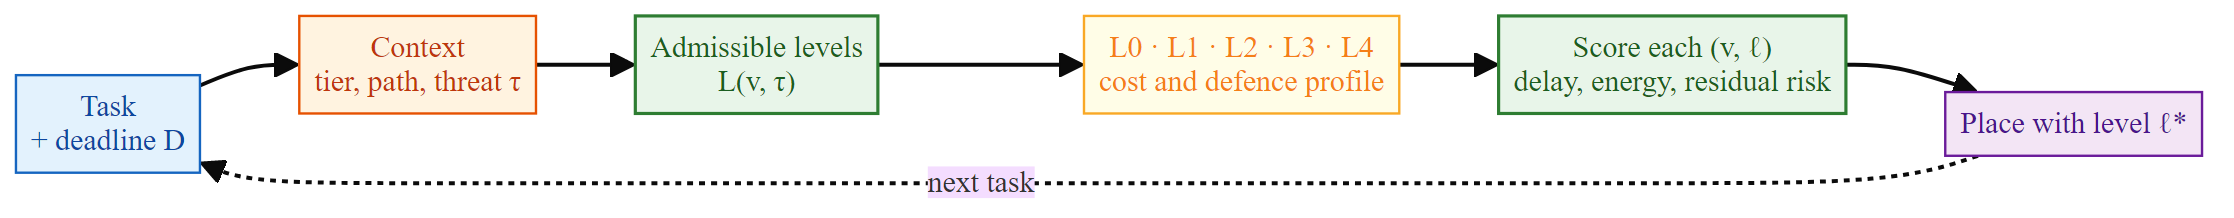
\includegraphics[width=0.66\textwidth]{security_loop.png}
\caption{Decision structure. The tier and the threat level restrict the admissible profile set; the orchestrator then scores every surviving $(v,\ell)$ pair on delay, energy and residual risk before applying the deadline constraint.}
\label{fig:model}
\end{figure*}

\subsection{Monotonicity}
\begin{proposition}[Profile monotonicity]
\label{prop:monotone}
If the defence factors are non-decreasing in the profile index and the cost
multipliers are non-decreasing, then for fixed $(\tau,\epsilon,s)$ the attack
probability \eqref{eq:composite} is non-increasing in $\ell$ and the expected
delay is non-decreasing in $\ell$.
\end{proposition}
\begin{IEEEproof}
Each channel probability in \eqref{eq:poison}--\eqref{eq:leak} is
non-increasing in the corresponding defence factor, and the defence factors are
non-decreasing in $\ell$ by assumption; the product in \eqref{eq:composite} is
therefore non-increasing in $\ell$. Delay is the sum of a compute term
proportional to the compute multiplier, a payload term proportional to the
payload multiplier, and the handshake latency, all non-decreasing in $\ell$.
\end{IEEEproof}
The proposition is elementary but it is the formal content of the trade-off:
the static profiles trace a monotone curve, and the adaptive policy is an
attempt to reach points off that curve by varying $\ell$ across tasks rather
than within them.

% =========================================================================
\section{Adaptive Orchestrator}
\label{sec:method}

\subsection{Admissible levels}
For a candidate node $v$ and task $i$ the orchestrator first computes an
admissible level set $\mathcal{L}(v,\tau)\subseteq\{0,\dots,4\}$. The set is
tier-dependent: a cloud placement, which crosses the shared WAN, is restricted
to L2--L4; an edge aggregation point is restricted to L2--L3 for ordinary tasks
and to L2--L4 for federated rounds; a mist peer is restricted to L2--L3. At
$\tau\le0.05$ the edge set collapses to L2, because there is no threat to
justify more.

The construction is a policy choice, not an optimisation result. Its purpose is
to encode the operational rule that the WAN is never used without a
post-quantum channel, which is exactly the rule an operator would write down
and exactly the rule that a static level assignment cannot express.

\subsection{Scoring and selection}
For each admissible pair the orchestrator estimates delay and energy in the
same way as a placement-only orchestrator, adding the profile's fixed
cryptographic instructions to the compute term, its fixed per-message kilobytes
to the payload term, and its handshake latency to the delay:
\begin{equation}
\hat D_i(v,\ell)=\frac{\tilde w_i(\ell)}{\mu_v}+Q_v+L_i(\tilde b_i(\ell))+h_\ell,
\label{eq:delay}
\end{equation}
where $\tilde w_i(\ell)=m_\ell w_i+c_\ell$ and
$\tilde b_i(\ell)=p_\ell b_i+d_\ell$ use the multipliers and fixed costs of
Table~\ref{tab:p4-crypto}. The score is a weighted sum of normalised delay,
energy, and residual risk,
\begin{equation}
J_i(v,\ell)=\frac{\hat D_i(v,\ell)}{D_i}+\lambda\frac{\hat E_i(v,\ell)}{E_0}
+\gamma\,p_{\text{attack}}(v,\ell,i),
\label{eq:score}
\end{equation}
subject to $\hat D_i(v,\ell)\le D_i$. If no pair satisfies the deadline, the
orchestrator falls back to the smallest predicted delay, because a task that
misses its deadline is worse than a task that is under-protected.

\begin{algorithm}[t]
\caption{Adaptive security-level and placement selection}
\label{alg:adaptive}
\begin{algorithmic}[1]
\Require task $i$, candidates $V$, threat $\tau$, weights $(\lambda,\gamma)$
\Ensure pair $(v^\ast,\ell^\ast)$
\State $best\gets\bot$;\quad $fallback\gets\bot$
\ForAll{$v\in V$}
  \State $\mathcal{L}\gets$ admissible levels of tier$(v)$ at $\tau$
  \ForAll{$\ell\in\mathcal{L}$}
    \State $\hat D\gets$ Eq.~\eqref{eq:delay};\quad $\hat E\gets$ energy$(\hat D)$
    \State $p\gets$ Eq.~\eqref{eq:composite}
    \State $J\gets\hat D/D_i+\lambda\hat E/E_0+\gamma p$
    \If{$\hat D\le D_i$ \textbf{and} $J<J(best)$} $best\gets(v,\ell)$ \EndIf
    \If{$\hat D<\hat D(fallback)$} $fallback\gets(v,\ell)$ \EndIf
  \EndFor
\EndFor
\State \Return $best$ if defined, else $fallback$
\end{algorithmic}
\end{algorithm}

\subsection{Complexity}
The inner loop runs over $|V|$ candidates and at most five levels, so the cost
per task is at most $5|V|$ delay estimations, each $\bigO(1)$ with cached queue
and route state. With $|V|\le33$ in our deployment the worst case is $165$
estimations per task, which is small compared with the simulator's own per-task
bookkeeping. No additional state is required beyond the per-tier level sets.

% =========================================================================
\section{Experimental Methodology}
\label{sec:exp}

\subsection{Simulator and workload}
Experiments run on the Python port of PureEdgeSim~\cite{mechalikh2021pureedgesim}.
The workload is the same three-class profile used in the companion agentic
study (Table~\ref{tab:p4-workload}): a hard real-time health class, a soft
real-time augmented-reality class, and a non-real-time heavy-compute class.
Thirty devices run for five simulated minutes, with the full mist/edge/cloud
architecture in all runs except the architecture column of the main grid.

\begin{table}[t]
\centering
\footnotesize
\caption{Workload classes (per generating device).}
\label{tab:p4-workload}
\begin{tabular}{@{}lccc@{}}
\toprule
 & Health & AR & Heavy\\
\midrule
Class & hard RT & soft RT & non RT\\
Rate (req/min) & 20 & 30 & 3\\
Deadline (s) & 0.02 & 0.50 & 300\\
Length (MI) & 500 & 5{,}000 & 30{,}000\\
Device share & 20\% & 30\% & 50\%\\
\bottomrule
\end{tabular}
\end{table}

\subsection{Policies and grids}
Six policies are compared: the five static profiles and \textsc{adaptive}. The
main grid crosses six policies with two architectures at threat $\tau=0.2$
($120$ runs). The attack grid crosses six policies with four threat levels
($240$ runs). The load grid crosses four policies (L0, L2, L4, adaptive) with
four arrival-rate factors ($160$ runs), and the size grid crosses the same four
policies with four model-size factors ($160$ runs). The total is $680$ runs,
ten seeds per cell.

Model size matters because the privacy-leakage term \eqref{eq:leak} scales with
the update size: a larger model is a larger inference surface, which is why
secure aggregation earns its cost at larger sizes and not at smaller ones.

\subsection{Statistics}
Comparisons use paired seeds, the Mann--Whitney $U$ test with Holm--Bonferroni
correction, bootstrap $95\%$ confidence intervals, and Cliff's $\delta$. The
determinism check re-ran one configuration and obtained identical values for
successes ($1{,}490$), mean delay ($0.2201$~s), energy ($13.5313$~Wh) and
composite attack rate ($0.1262$).

% =========================================================================
\section{Results}
\label{sec:res}

\subsection{The price of unconditional security}
Table~\ref{tab:p4-main} reports the main grid at $\tau=0.2$. Read the delay
column first: L0 takes $0.226$~s, L4 takes $0.469$~s, and the intermediate
profiles are ordered by their multipliers. The relative overhead column makes
the jump explicit: $+19.8\%$ for a signature, $+22.4\%$ for a post-quantum
channel, $+63.6\%$ for adding homomorphic encryption, $+107.9\%$ for adding
secure aggregation. Byte amplification follows the same order, from $1.00\times$
to $2.06\times$, because ciphertext expansion is the dominant cost of the
upper levels.

Read the attack column second. L0 admits a composite attack rate of $0.415$,
L1 reduces it to $0.315$, L2 to $0.164$, L3 to $0.059$, L4 to $0.019$. The
reduction per unit of delay is highly non-uniform: L1 buys a quarter of the
total reduction for a fifth of the total delay cost, while the step from L3 to
L4 buys a further $0.040$ for another $0.044$~s. A deployment with no
per-exchange control must pick one of these points, and every choice is wrong
for some of its traffic.

Success ratio is almost flat across profiles ($0.988$--$1.000$), which is worth
noting: the cryptographic overhead does not cost throughput on this workload
because the deadlines are loose enough to absorb it. The cost appears in delay
and bytes, not in completed work. A study that reported only success would
conclude that security is free.

\begin{table*}
\centering
\small
\caption{Performance and security outcomes across security levels, adaptive policy, and architectures (mean of 10 seeds, threat = 0.20).}
\label{tab:p4-main}
\begin{tabular}{llccccccc}
\toprule
Architecture & Policy & Success & Delay (s) & Delay ovh. & Wh/succ. & Byte amp. & Attack rate & Prot. utility \\
\midrule
ALL & adaptive & 1.000 & 0.234 & +3.7\% & 0.009 & 1.23x & 0.126 & 0.874 \\
ALL & level0 & 0.992 & 0.226 & +0.0\% & 0.009 & 1.00x & 0.415 & 0.580 \\
ALL & level1 & 0.993 & 0.270 & +19.8\% & 0.009 & 1.05x & 0.315 & 0.680 \\
ALL & level2 & 0.992 & 0.276 & +22.4\% & 0.009 & 1.23x & 0.164 & 0.829 \\
ALL & level3 & 0.989 & 0.369 & +63.6\% & 0.009 & 1.66x & 0.059 & 0.931 \\
ALL & level4 & 0.988 & 0.469 & +107.9\% & 0.010 & 2.06x & 0.019 & 0.970 \\
EDGE\_AND\_CLOUD & adaptive & 1.000 & 0.238 & +10.1\% & 0.009 & 1.23x & 0.125 & 0.875 \\
EDGE\_AND\_CLOUD & level0 & 0.989 & 0.216 & +0.0\% & 0.009 & 1.00x & 0.415 & 0.578 \\
EDGE\_AND\_CLOUD & level1 & 0.989 & 0.237 & +9.4\% & 0.009 & 1.05x & 0.315 & 0.677 \\
EDGE\_AND\_CLOUD & level2 & 0.988 & 0.248 & +14.4\% & 0.009 & 1.23x & 0.164 & 0.826 \\
EDGE\_AND\_CLOUD & level3 & 0.988 & 0.337 & +55.5\% & 0.010 & 1.66x & 0.059 & 0.930 \\
EDGE\_AND\_CLOUD & level4 & 0.986 & 0.428 & +97.6\% & 0.010 & 2.06x & 0.018 & 0.968 \\
\bottomrule
\end{tabular}
\par\vspace{2pt}{\footnotesize\raggedright Delay ovh. is relative to L0 (none); Prot. utility = success ratio $\times$ (1 $-$ composite attack rate).\par}
\end{table*}


\begin{figure*}[t]
\centering
\begin{subfigure}[b]{0.32\textwidth}
  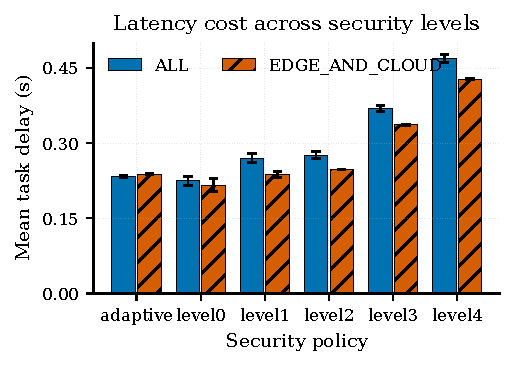
\includegraphics[width=\linewidth]{f2_delay_by_level.pdf}
  \caption{Mean delay.}
\end{subfigure}\hfill
\begin{subfigure}[b]{0.32\textwidth}
  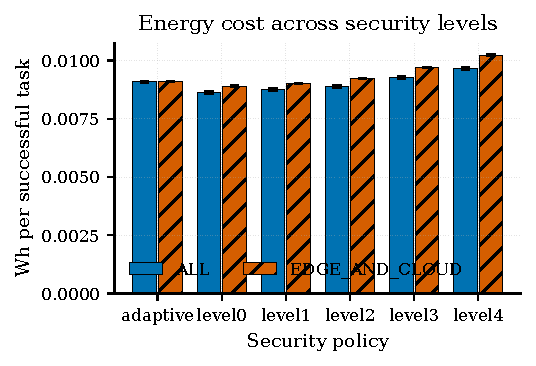
\includegraphics[width=\linewidth]{f2b_energy_by_level.pdf}
  \caption{Energy per task.}
\end{subfigure}\hfill
\begin{subfigure}[b]{0.32\textwidth}
  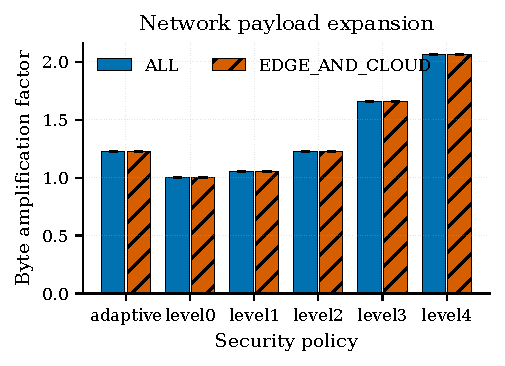
\includegraphics[width=\linewidth]{f2c_bytes_by_level.pdf}
  \caption{Bytes per task.}
\end{subfigure}
\caption{Cost of the static profiles, with $95\%$ confidence intervals. Delay
and bytes grow monotonically with the profile; energy is nearly flat because
the cryptographic work is a small fraction of the compute budget.}
\label{fig:cost}
\end{figure*}

\subsection{Adaptive is Pareto-optimal, not dominant}
Fig.~\ref{fig:pareto} places the six policies on the delay--utility plane.
Adaptive sits at $(0.234~\text{s}, 0.874)$; L2 at $(0.276,0.829)$; L1 at
$(0.270,0.680)$; L0 at $(0.226,0.580)$; L3 at $(0.369,0.931)$; L4 at
$(0.469,0.970)$. Three statements follow, and only three.
First, adaptive \emph{dominates} L1 and L2: it is both faster and more secure
than either. Second, adaptive \emph{does not dominate} L3 or L4: both achieve
higher utility, and a deployment that values utility above delay should choose
L4 and accept $+107.9\%$. Third, adaptive \emph{is not dominated by} any static
profile: no static point is both faster and more secure, so it lies on the
Pareto front.

The same ordering holds under \textsc{edge\_and\_cloud}, with adaptive at
$(0.238,0.875)$ and L4 at $(0.428,0.968)$, so the conclusion does not depend on
whether the mist tier participates.

\begin{table*}
\centering
\small
\caption{Non-parametric comparisons of adaptive security against unprotected (L0) and static max-security (L4) baselines (10 seeds, Mann--Whitney $U$).}
\label{tab:p4-tests}
\begin{tabular}{lcccccc}
\toprule
Metric & Control & Treatment & Difference & 95\% CI & Cliff's $\delta$ \\
\midrule
task\_delay\_mean\_s (vs L0) & 0.226 & 0.234 & 0.008 & [0.000, 0.017] & 0.32 \\
task\_delay\_mean\_s (vs L4) & 0.469 & 0.234 & -0.235$^{**}$ & [-0.243, -0.228] & -1.00 \\
energy\_per\_success\_wh (vs L0) & 0.009 & 0.009 & 0.000$^{**}$ & [0.000, 0.000] & 1.00 \\
energy\_per\_success\_wh (vs L4) & 0.010 & 0.009 & -0.001$^{**}$ & [-0.001, -0.001] & -1.00 \\
security\_composite\_attack\_rate (vs L0) & 0.415 & 0.126 & -0.289$^{**}$ & [-0.290, -0.288] & -1.00 \\
security\_composite\_attack\_rate (vs L4) & 0.019 & 0.126 & 0.108$^{**}$ & [0.107, 0.108] & 1.00 \\
protected\_utility (vs L0) & 0.580 & 0.874 & 0.294$^{**}$ & [0.293, 0.294] & 1.00 \\
protected\_utility (vs L4) & 0.970 & 0.874 & -0.096$^{**}$ & [-0.098, -0.094] & -1.00 \\
\bottomrule
\end{tabular}
\par\vspace{2pt}{\footnotesize\raggedright Holm--Bonferroni adjusted: $^{*}p<0.05$, $^{**}p<0.01$, $^{***}p<0.001$. CI = bootstrap 95\% confidence interval of the difference.\par}
\end{table*}


Table~\ref{tab:p4-tests} quantifies the two comparisons. Against L0, adaptive
costs $+0.008$~s of mean delay (confidence interval $[0.000,0.017]$, Cliff's
$\delta=0.32$, not significant), $+0.000$~Wh per success, and buys a $0.289$
reduction in attack rate and a $0.294$ increase in protected utility, both with
$\delta=-1.00$ and $1.00$ respectively. Against L4, adaptive saves $0.235$~s of
mean delay, $0.001$~Wh per success, and gives up $0.108$ of attack protection
and $0.096$ of utility, all with $\delta=\pm1.00$. The comparisons are
deliberately symmetric: one shows what protection buys, the other what it
costs.

\begin{figure}[t]
\centering
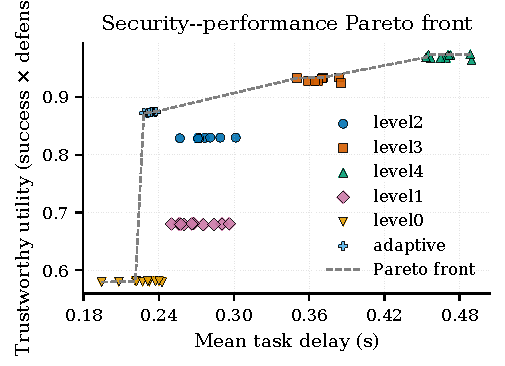
\includegraphics[width=\columnwidth]{f3_pareto_utility.pdf}
\caption{Delay--utility plane. Adaptive lies on the Pareto front: it dominates
the two middle profiles and is not dominated by the upper ones, which are
slower and more secure.}
\label{fig:pareto}
\end{figure}

\subsection{Robustness across threat levels}
Table~\ref{tab:p4-attack} and Figs.~\ref{fig:attack}(a)--(b) sweep the threat
intensity from $0$ to $0.4$. The unprotected curve falls steeply, from $0.848$
to $0.367$; the adaptive curve falls gently, from $0.935$ to $0.814$; the L4
curve is almost flat, from $0.981$ to $0.959$. The slopes are the result: a
static low-security profile is viable only when the threat is low, and a static
high-security profile is viable at any threat but pays its delay at all of
them. Adaptive tracks the threat, which is what a policy with a threat input
should do.

The ordering at $\tau=0.4$ is L4 $(0.959)$, L3 $(0.893)$, adaptive $(0.814)$,
L2 $(0.750)$, L1 $(0.524)$, L0 $(0.367)$. Adaptive is third, as at every threat
level, and its gap to L3 narrows slightly as the threat rises because the
orchestrator escalates the levels it chooses. It never closes, because adaptive
still refuses the L4 profile on delay-sensitive tasks.

Fig.~\ref{fig:attack}(b) isolates the privacy channel. The
membership-inference leakage proxy rises with the threat for every policy, and
it is the channel that the adaptive policy controls least well: the effective
defence is secure aggregation, which only L4 provides, and L4 is the profile the
orchestrator refuses on delay-sensitive tasks. The size sweep in
Fig.~\ref{fig:loadsize}(b) confirms the dependence on update size that
\eqref{eq:leak} encodes. This is the clearest single weakness of the policy and
we return to it in Section~\ref{sec:disc}.

\begin{table*}
\centering
\small
\caption{Trustworthy utility across adversarial threat intensities $\tau \in \{0, 0.1, 0.2, 0.4\}$.}
\label{tab:p4-attack}
\begin{tabular}{lcccccc}
\toprule
threat\_level & adaptive & level0 & level1 & level2 & level3 & level4 \\
\midrule
0.000 & 0.935 & 0.848 & 0.863 & 0.913 & 0.969 & 0.981 \\
0.100 & 0.904 & 0.707 & 0.768 & 0.870 & 0.950 & 0.976 \\
0.200 & 0.874 & 0.580 & 0.680 & 0.829 & 0.931 & 0.970 \\
0.400 & 0.814 & 0.367 & 0.524 & 0.750 & 0.893 & 0.959 \\
\bottomrule
\end{tabular}
\end{table*}


\begin{figure*}[t]
\centering
\begin{subfigure}[b]{0.48\textwidth}
  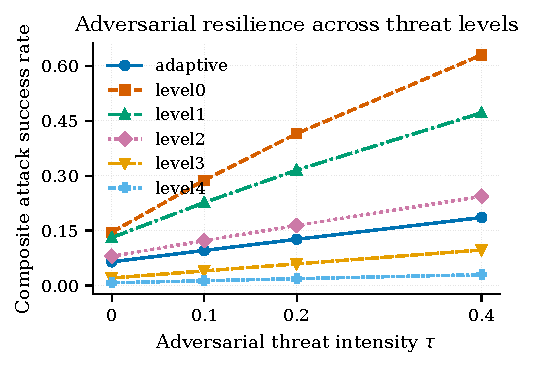
\includegraphics[width=\linewidth]{f4_attack_vs_threat.pdf}
  \caption{Composite attack rate versus threat intensity.}
\end{subfigure}\hfill
\begin{subfigure}[b]{0.48\textwidth}
  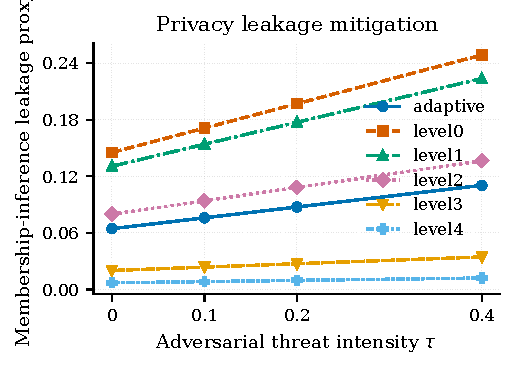
\includegraphics[width=\linewidth]{f4b_privacy_leakage.pdf}
  \caption{Privacy leakage by profile.}
\end{subfigure}
\caption{Threat sweep. Adaptive degrades gracefully between the unprotected
baseline and maximum security; the privacy channel is where it lags most.}
\label{fig:attack}
\end{figure*}

\subsection{Load and model size: where the ranking inverts}
Figs.~\ref{fig:loadsize}(a) and~(b) stress the policy along two axes that
interact with cryptography, and both produce a ranking that differs from the
main grid.

Under load, the four policies do not move together. The unprotected and
lightly protected policies are almost flat: L0 moves from $0.577$ to $0.584$ and
L2 from $0.823$ to $0.830$ as the arrival rate grows four-fold. L4 rises to
$0.951$ at $2\times$ and then collapses to $0.729$ at $4\times$, because its
delay grows to $0.688$~s and deadline failures enter the utility product. The
adaptive policy holds $0.874$ up to $2\times$ and falls to $0.736$ at $4\times$.
At saturation L2 has the highest utility of the four ($0.830$), so the correct
response to overload is to \emph{de-escalate} the profile, which the fixed
risk weight of \eqref{eq:score} does not do. We report this as a limitation
rather than tuning the weight after seeing the result.

Under model size the inversion is sharper. At $4\times$ the update size, L4's
utility falls from $0.970$ to $0.043$ as its delay grows from $0.469$~s to
$2.327$~s; L2 falls to $0.350$; adaptive falls to $0.439$; and even the
unprotected policy falls to $0.519$, because a larger update costs transfer
time even without cryptography. At that scale the unprotected policy has the
highest utility of the four, which is a statement about our workload's
sensitivity profile, not a recommendation. What generalises is the ordering of
the losses: protection becomes relatively more expensive as the update grows,
because the payload multiplier applies to a larger object.

Taken together the two sweeps say that the profile should depend on load and
model size, not only on threat. Our orchestrator conditions on threat and tier
but not on the current utilisation, which is exactly why it is overtaken at
$4\times$ load. Adding a utilisation term to the admissible-level construction
is the obvious next iteration and is cheap: the queue state is already an input
to the delay estimate.

\begin{figure*}[t]
\centering
\begin{subfigure}[b]{0.48\textwidth}
  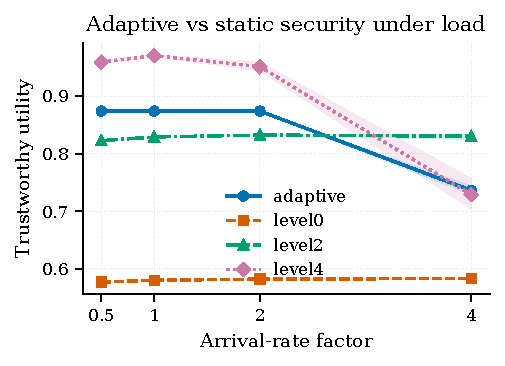
\includegraphics[width=\linewidth]{f5_load_utility.pdf}
  \caption{Utility versus arrival-rate factor.}
\end{subfigure}\hfill
\begin{subfigure}[b]{0.48\textwidth}
  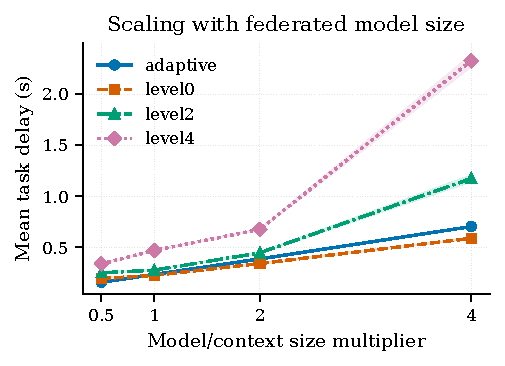
\includegraphics[width=\linewidth]{f5b_model_size_delay.pdf}
  \caption{Delay versus model-size factor.}
\end{subfigure}
\caption{Load and model-size sweeps. Both axes move the ranking of profiles:
under saturation the cheap profiles win, and at large update sizes the delay of
the strongest profile grows fastest.}
\label{fig:loadsize}
\end{figure*}

\subsection{Where the overhead goes}
Fig.~\ref{fig:breakdown} decomposes the per-task overhead into cryptographic
compute (MI), network bytes, and container footprint. The decomposition shows
that the three components do not scale together: compute overhead is roughly
linear in the profile index, byte overhead grows faster because ciphertext
expansion compounds with the payload multiplier, and container overhead grows
slowest because it depends on the container multiplier rather than the payload
one. For L4 the byte term dominates, which is why the orchestrator's preference
for edge-local aggregation matters: moving a federated round from the WAN to the
edge removes the dominant term from the expensive path.

\begin{figure}[t]
\centering
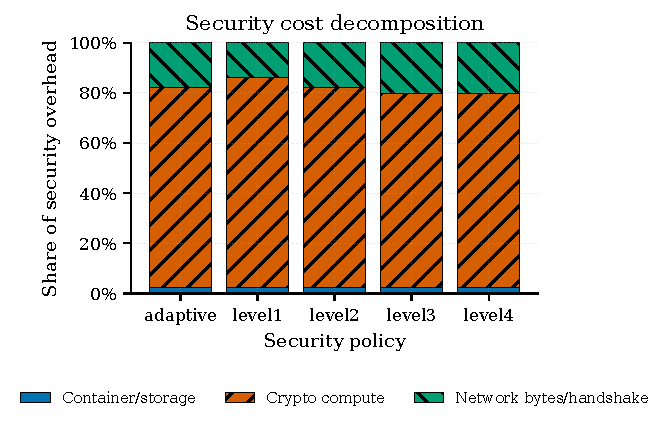
\includegraphics[width=\columnwidth]{f6_overhead_breakdown.pdf}
\caption{Overhead decomposition by profile. The byte term dominates at the upper
levels, which is what motivates edge-local aggregation.}
\label{fig:breakdown}
\end{figure}

\subsection{Summary}
Four findings. (i) Unconditional maximum security costs $+107.9\%$ delay and
$2.06\times$ bytes to reduce the attack rate from $0.415$ to $0.019$. (ii) The
adaptive policy reaches $0.126$ at $+3.7\%$, which is $69.6\%$ of the attack
reduction for $3.4\%$ of the delay cost. (iii) Adaptive is Pareto-optimal and
dominates the two middle profiles, but it is third on protected utility behind
L3 and L4. (iv) The ranking is not universal: at $4\times$ load the cheap L2
profile has higher utility than adaptive, and at $4\times$ model size even the
unprotected policy does, which bounds the claim to the nominal-to-moderate
regime.

% =========================================================================
\section{Discussion}
\label{sec:disc}

\emph{Why a frontier and not a winner.} The security--performance trade is not
a problem with a single optimum; it is a menu. An operator with a hard
$50$~ms budget must choose the adaptive policy or nothing; an operator
protecting medical model updates should choose L4 and buy more hardware. The
contribution of an orchestrator is to make the menu available per exchange,
not to pick a point for everyone.

\emph{Why adaptive never reaches L4's utility.} The admissible-level sets
exclude L4 on edge nodes for non-federated tasks and on mist nodes entirely,
and the score penalises delay heavily. Both choices are deliberate: L4 costs a
handshake of $22$~ms alone, which exceeds the $20$~ms health deadline before any
compute happens. A policy that allowed L4 for that class would report higher
utility on paper and miss every deadline in practice. The gap to L4 is
therefore the price of respecting deadlines, and it is visible rather than
hidden.

\emph{The privacy gap.} Membership inference is the channel that the
orchestrator handles least well, because the effective defence is secure
aggregation and the effective alternative---homomorphic encryption---costs
$1.65\times$ payload. A deployment whose dominant risk is inference should
raise $\gamma$, the risk weight, which shifts the choice toward L3/L4 at the
cost of delay. The weight is exposed for exactly this reason.

% =========================================================================
\section{Threats to Validity}
\label{sec:threats}

\paragraph{Modelled, not implemented, cryptography}
The simulator executes no cryptographic code. The costs in
Table~\ref{tab:p4-crypto} are multipliers and fixed instruction counts
calibrated from the standards and the cited papers; they are defensible as
orders of magnitude and as relative costs, not as measurements on a specific
platform. A real ML-KEM encapsulation on a constrained device may be faster or
slower than our $1{,}150$~MI by a factor of two.

\paragraph{No formal security guarantee}
The attack model \eqref{eq:poison}--\eqref{eq:composite} is a probabilistic
proxy, not a reduction. It says nothing about whether ML-KEM or CKKS is
implemented correctly, nothing about side channels, and nothing about adaptive
attackers who observe the policy's own level choices. The defence factors are
calibrated estimates. A reader should treat the attack rates as a comparative
index, not as guarantees.

\paragraph{Construct validity of protected utility}
$U=\text{success}\times(1-\overline{p_{\text{attack}}})$ weights a missed
deadline and an attack equally at the margin. A deployment that considers a
privacy breach an order of magnitude worse than a late response would rank the
profiles differently. The metric is stated explicitly so that the reader can
recompute the ranking under a different weighting.

\paragraph{External validity}
Thirty devices, three application classes, two architectures, one threat
parameterisation. The threat levels are scalars, whereas a real adversary has a
capability profile. The workload is the same proxy profile used in the
companion agentic study, so the absolute delays are not transferable to a
GPU-equipped edge.

\paragraph{Conclusion validity}
Ten seeds per cell support the large effects ($\delta=\pm1.00$) and not the
small ones; the adaptive-versus-L0 delay difference is reported as
non-significant, which is the correct reading. The determinism check covers one
configuration.

% =========================================================================
\section{Conclusion}
\label{sec:concl}

We formalised five literature-calibrated security profiles, an adversary with
poisoning, eavesdropping and inference channels, and an orchestrator that
selects the profile and the host jointly under a deadline constraint. Across
$680$ seeded runs, unconditional maximum security costs $+107.9\%$ delay and
$2.06\times$ bytes for an attack rate of $0.019$; no protection gives $0.415$
for free; the adaptive policy achieves $0.126$ at $+3.7\%$ delay, which is
$69.6\%$ of the protection for $3.4\%$ of the cost.

The adaptive policy is Pareto-optimal and dominates the two middle static
profiles on both delay and utility. It is third on protected utility behind the
two strongest static profiles, and we have been explicit about that rather than
choosing a baseline that flatters it. The remaining gap is the price of
respecting deadlines: the strongest profile's handshake alone exceeds the
tightest deadline in the workload.

The next steps are to replace the multiplier calibration with measurements on a
representative edge platform, to extend the adversary to one that observes the
policy's level choices, and to price privacy breaches asymmetrically so that the
utility metric reflects a deployment's actual loss function.

\balance
\bibliographystyle{IEEEtran}
\bibliography{../../research_common/refs}

\end{document}
